
\chapter{The Gram Schmidt Walk Algorithm}
\label{ch:gram-schmidt}
We now give an efficient algorithm for Banaszczyk's result as stated
in Theorem \ref{thm:bana} (assuming access to a membership oracle for
the convex set $K$).
As discussed in Section \ref{sec:bana-core}, it is not clear how to
work directly with a general $K$ or use the arguments in
Chapter~\ref{ch:bana-proof} or Chapter~\ref{ch:algo-komlos-bana} to give an algorithm. 

Instead we will use the following equivalent formulation described in Section \ref{sec:bana-subgaussian}. 


%We state this again for convenience.

\begin{theorem}
\label{thm:bana-subgaussian2}
Given arbitrary vectors $v_1,\ldots,v_n \in \R^m$ with
$\|v_i\|_2 \leq 1$, there is a distribution $D$ over colorings
$x \in \{-1,1\}^n$ such that the resulting discrepancy vector
$\sum_{j=1}^n x(j) v_j$, where $x$ is sampled from $D$, has a
mean-zero $O(1)$-sub-Gaussian distribution.

Moreover, given $v_1, \ldots, v_n$, a coloring $x$ can be sampled from
$D$ in polynomial time.
\end{theorem}

We will describe a randomized algorithm called the Gram-Schmidt Walk (GS Walk), that given $v_1,\ldots,v_n$ produces a random  coloring $x$ (sampled from some implicit distribution $D$) such that the resulting discrepancy vector $Y$ is $\sqrt{20}$-sub-Gaussian.


\smallskip 
Before describing the algorithm, it is instructive to consider the following two examples to get some intuition for the sub-Gaussianity condition in Theorem \ref{thm:bana-subgaussian2}. %The following  two examples are quite instructive.

\begin{example}
\label{ex:gs-1}
    Suppose that $v_1,\ldots,v_n$ are orthogonal unit vectors. 
    
    We claim that in this case, a uniformly random $\pm 1$ coloring suffices. Indeed fix some vector $\theta \in \R^m$. Then  
    \[\ip {\theta,Y}=
\ip {\theta, \sum_{j=1}^n x(j) v_j} = \sum_{j=1}^n  x(j) \ip{\theta,v_j}.\]
For a uniformly random coloring $x \in \{-1,1\}^n$, each $x(j)$ is an
independent and uniform sample in $\{-1,+1\}$, and hence $x(j) \ip{\theta,v_j}$
is $O(|\ip{\theta,v_j}|)$-sub-Gaussian by Hoeffding's lemma. By
independence $\sum_{j=1}^n  x(j) \ip{\theta,v_j}$ is $\sigma$-sub-Gaussian
with $\sigma\lesssim \sqrt{\sum_{j=1}^n \ip{ \theta, v_j}^2 }$, and the
right hand side is at most $ \|\theta\|_2$  as the $v_j$ are orthonormal.

\begin{remark}
    The randomness is crucial; if we just output a fixed coloring $x$,
    then $Y=\sum_{j=1}^n x(j)v_j$ is $\sqrt{n}$-sub-Gaussian as
    $\ip{Y,\theta} = \|Y\|_2 = \sqrt{n}$ for the unit vector $\theta = Y/\|Y\|_2$.
\end{remark} 
\end{example} 

 \begin{example}
 \label{ex:gs-2}
On the other extreme, suppose that $v_1 = \cdots = v_n =v $ are all
identical to some $v$ with $\|v\|_2=1$. Then a uniformly random
coloring is  very bad as $Y = \left(\sum_{j=1}^n x(j)\right) v$, and
\(
  \E [\ip{Y,\theta}^2] = \E\left(\sum_{j=1}^n x(j)\right)^2 = n
\)
for
$\theta =v$, while we require that $\E [\ip{Y,\theta}^2] \lesssim
1$ for an $O(1)$-sub-Gaussian $Y$ and a unit vector $\theta$.
%(in fact for any $\theta = \alpha v$).

The right thing to do in this example, of course, is to pair up the
signs $x(j)$ and cancel them out as much as possible. We can
then make sure that $\|Y\|_2 \lesssim 1$ with probability $1$.
%In other words, for random coloring $Y$ is typically $\Theta(\sqrt{n})v$, while we require it to be $O(1)v$.
\end{example}

The GS Walk algorithm will handle these two extreme scenarios in a unified way. It will exploit the linear dependencies to cancel things exactly as much as possible, and at the same time have enough randomness so that  the resulting distribution is $O(1)$-sub-Gaussian.

We describe this algorithm next in Section~\ref{sec:gs:algorithm}.
In Section~\ref{sec:gs-covariance} we show that the covariance of the output discrepancy vector $Y$ satisfies $\text{Cov}(Y) \preceq I$ and finally in Section~\ref{sec:gs-subgaussian} we prove the sub-Gaussianity.

\section{The Gram-Schmidt Walk}
\label{sec:gs:algorithm}
We first describe the algorithm informally.

Let $v_1,\ldots,v_n \in \R^m$ be the input vectors. The algorithm begins with the fractional coloring $x_0 =(0,\ldots,0)$ and updates it iteratively over time until the final coloring $x_T \in \{-1,1\}^n$. Once  a coordinate reaches $\pm 1$ it is frozen and not updated anymore, otherwise it is alive.

To update the coloring at time $t$, we compute an update direction
$u_t$ based on which coordinates are still alive, and set $x_t = x_{t-1} + \delta_t u_t$ where the step size $\delta_t$ is chosen randomly such that $\E[\delta_t]=0$ and at least one new variable gets frozen.

\paragraph{Computing the update.} The idea behind the update step (which is the crux of the algorithm) is the following. 

Assume for simplicity that no coordinate is frozen.
Let $B$ denote the matrix with columns $v_1,\ldots,v_n$. 
If the coloring $x$ is updated by $u$, the discrepancy vector changes by $Bu = u(1) v_1 + u(2) v_2 +  \ldots + u(n) v_n$.

Suppose that we are required to set $u(n)=1$ (to ensure progress on coordinate $n$),   
but can freely set $u(1),\ldots,u(n-1)$ in $\R$ (not just in  $[-1,1]$). Then intuitively, we should try to use this flexibility to cancel things to to make $Bu$ as small as possible. 

Concretely, let us try to minimize $\|Bu\|_2$ subject to $u(n) = 1$.
Then we explicitly have
\begin{align}
\label{eq:gs-bu}
    \min_{u: u(n)=1} \| Bu\|_2 & =  \min_{u(1),\ldots,u(n-1) } \left\|v_n  + \sum_{j=1}^{n-1} u(j) v_j  \right\|_2  \nonumber \\
    & = \|\Pi_{V^\perp} (v_n)\|_2,
\end{align} 
%We now describe the algorithm formally.
where $V=\text{span}(v_1,\ldots,v_{n-1})$ is the subspace spanned by $v_1,\ldots,v_{n-1}$, $V^\perp$ is the subspace orthogonal to $V$, and for any subspace $W$, $\Pi_W$ denotes the orthogonal projection operator onto  $W$. 

To see \eqref{eq:gs-bu}, set $u(1),\ldots,u(n-1)$ so that
$\sum_{i=1}^{n-1} u(i) v_i = - \Pi_V(v_n)$ and hence $Bu = v_n -
\Pi_V(v_n) =\Pi_{V^\perp} (v_n)$. This is also
the least possible value of $\|Bu\|_2$, because $\sum_{j=1}^{n-1} u(j)
v_j \in V$, so
\[
  \|Bu\|_2 \ge \|\Pi_{V^\perp}(Bu)\|_2 = \|\Pi_{V^\perp} (v_n)\|_2.
\]

\paragraph{Notation.}
 The algorithm is described formally below. See also Figure \ref{fig:enter-label}.
Let $x_{t-1}$ and $ A_{t-1}$ denote the coloring and the set of alive coordinates at the beginning of time $t$. 
Let
 $p_t$ be the largest-indexed (alive) element in $A_{t-1}$ at time $t$. 
 
 We compute the vector $u_t$ to achieve the minimum in \eqref{eq:gs-bu} (restricted to alive coordinates and $p_t$ as the index $n$), and update $x_t$ randomly along $u_t$
 so that $x_t$ stays in $[-1,1]^n$ and least one more variable reaches $\pm 1$.
 We call $p_t$ the \textit{pivot}  at time $t$, and it plays a special role at time $t$.
 



\begin{figure}[hbtp!]
    \centering
    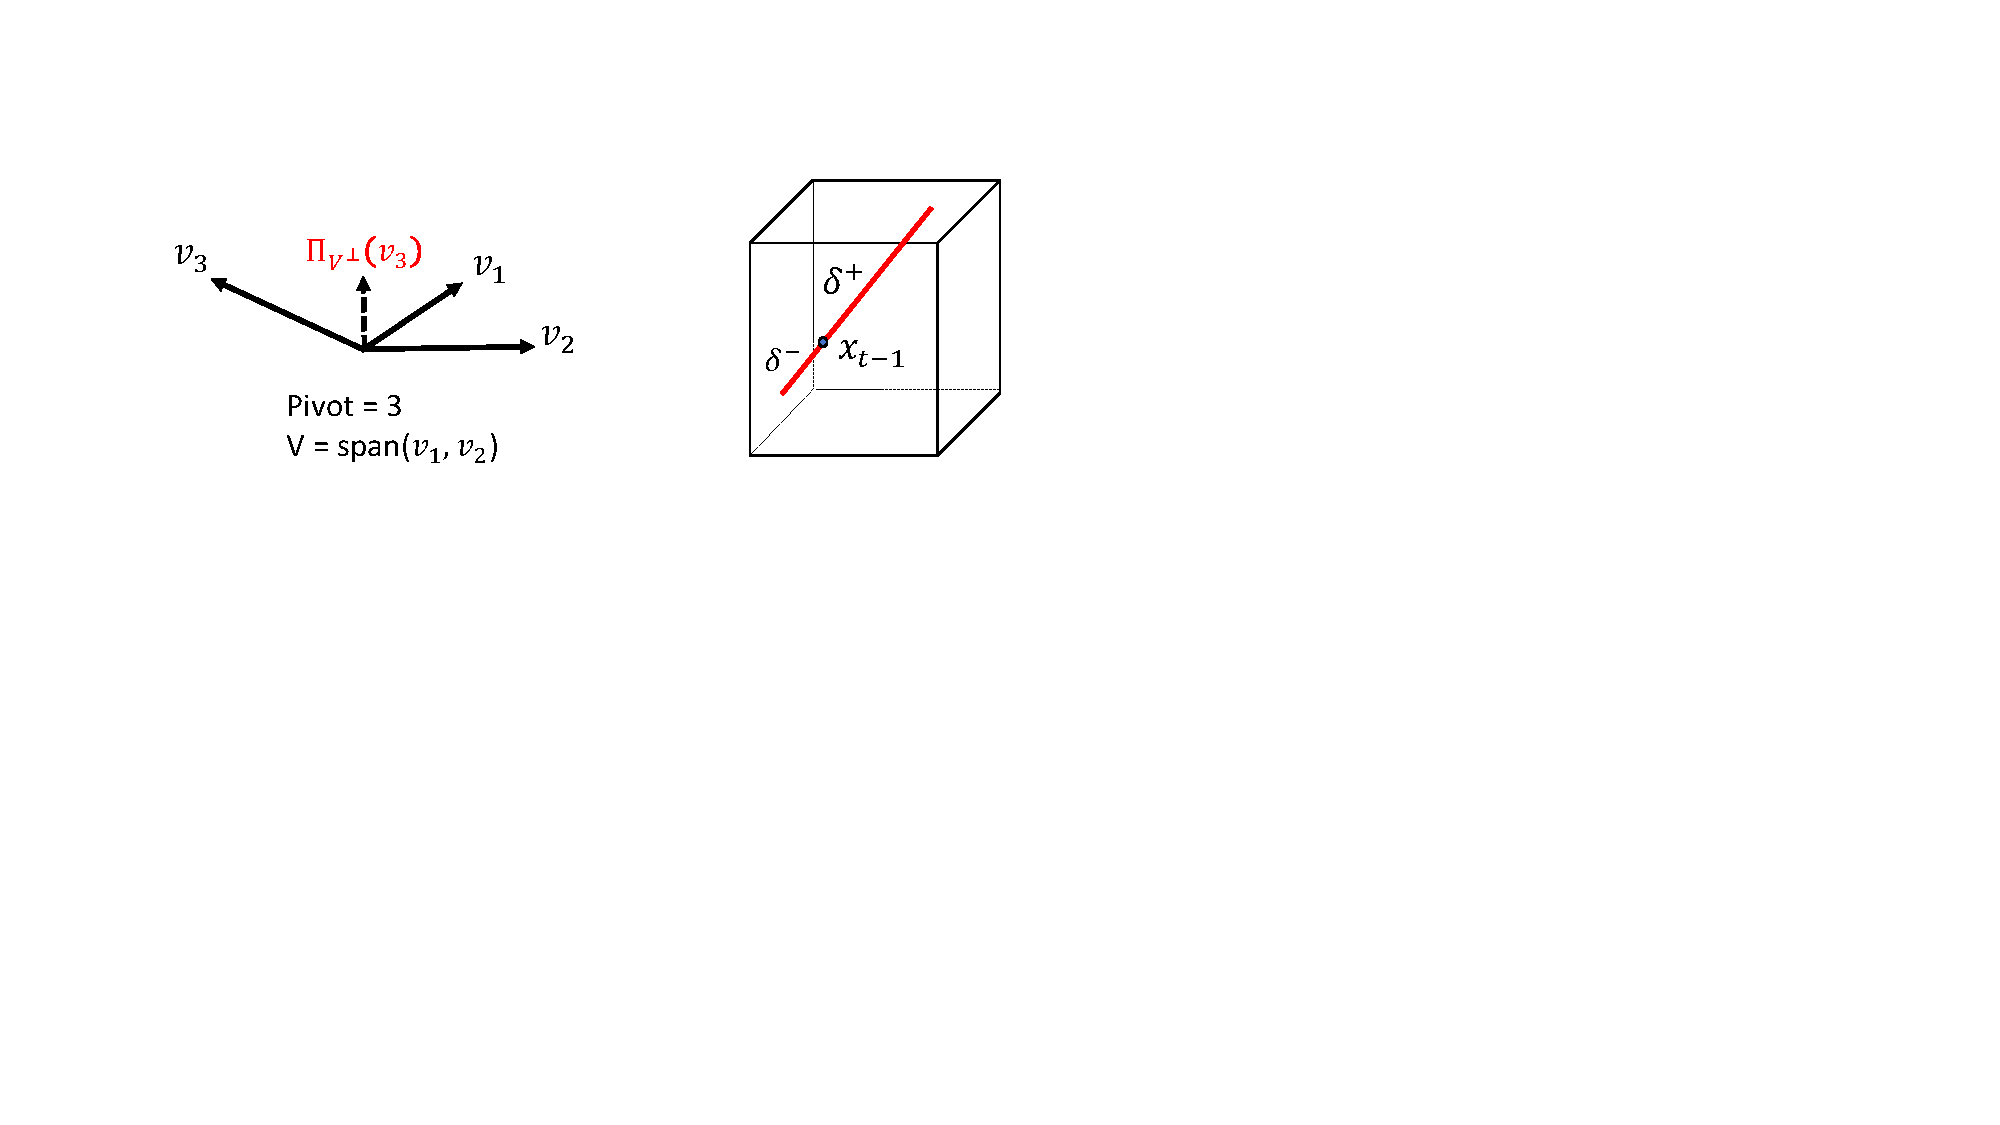
\includegraphics[scale=0.7, trim=5mm 10mm 20mm 5mm]{gs.pdf}
    \caption{The left shows the pivot and discrepancy update direction. The right shows how the coloring updates.}
    \label{fig:enter-label}
\end{figure} 


\noindent {\bf Algorithm Description.} 
Let $B$ denote the input matrix with columns $v_1,\ldots,v_n$. 
Initialize $x_0=(0,\ldots,0)$ and $A_0=[n]$.\\

For $t=1,\ldots,n$ do the following:
\begin{enumerate}

\item 
Compute  $u_t = \text{argmin}_{u} \|Bu\|_2$, subject to $u(p_t)=1$ for the pivot $p_t$, and $u(j)=0$ for each frozen variable $j \notin A_{t-1}$.

\item Let $\delta^{-}_t <0< \delta^{+}_t$ be the maximal negative and positive values for $\delta$, such that 
$|x_{t-1} + \delta u_t| \in [-1, 1]^n$ for all $\delta \in
[\delta_t^-, \delta_t^+]$.
%$\|(x_{t-1}+\delta u_t)_{A_t}\|_\infty=1$ \ddnote{Need to restrict to coordinates in $A_t$}.
Let
%$\delta_t \in \{\delta^{-}_t,\delta^{+}_t\}$ is chosen randomly as
\[
\delta_t \eqdef
\begin{cases}
\delta^{-}_t & \text{with probability }  \delta^{+}_t/(\delta^{+}_t -  \delta^{-}_t)\\
\delta^{+}_t & \text{with probability }  -\delta^{-}_t/( \delta^{+}_t -  \delta^{-}_t)
\end{cases}\;.
\]
\item Set $x_t = x_{t-1} + \delta_t u_t$, and update $A_t \eqdef \{i \in [n]: |x_t(i)| < 1\}$.
%\item Update $A_{t+1} = \{i \in [n]: |x_t(i)| < 1\}$, $n(t+1) = \max \{i %\in
%A_{t+1}\}$ and $t \leftarrow t+1$.
\end{enumerate}
%\item Output $x_t$.
%\end{enumerate}


\subsection{Basic Properties}
Let us note some basic properties of the algorithm and define some notation that will be useful later.
\paragraph{Coloring update.}
Let $\Delta x_t := x_t - x_{t-1} = \delta_t u_t$ denote the coloring update  at time $t$, and
let $\Omega_{t-1}$ denote all the random choices $\delta_1,\ldots,\delta_{t-1}$ made by the algorithm  by time $t-1$.
Note that $\E[\delta_t| \Omega_{t-1}]=0$, and thus each color $x_t(i)$ evolves as a martingale. 

The step sizes $\delta_t^-,\delta_t^+$  ensure that at least one alive variable always reaches $\pm 1$.
%while keeping $x_t$ in $[-1,1]^n$. 
We can assume that exactly one variable gets frozen per step (else we can divide the step into several steps). Thus the algorithm terminates in exactly $n$ steps. 

\paragraph{Discrepancy update.} Let $d_t := Bx_t$ denote the discrepancy vector at the end of time $t$, and let
$\Delta d_t := d_t - d_{t-1}$ denote its update at $t$.

At time $t$, let $V_t$ denote the subspace spanned by the alive vectors excluding the pivot, that is by $\{ v_i:i \in A_{t-1}, i \neq  p_t\}$. 
%It will be useful to further decompose $\Pi_{V_t^\perp}(v_{p(t)}$.
Notice that $V_0 \supseteq V_1 \supseteq \ldots \supseteq V_n = \emptyset$, is a (random) nested sequence produced by the execution of the algorithm, where we define $V_0= \text{span}\{v_1,\ldots,v_n\}$.
Equivalently, $V_0^\perp \subseteq V_1^\perp \subseteq \ldots \subseteq V_n^\perp$.

As $Bu_t = \Pi_{V_t^\perp}(v_{p_t})$ by \eqref{eq:gs-bu}, we can explicitly write
\begin{equation}
\label{eq:gs-disc-update-explicit1}
    \Delta d_t = B \Delta x_t =  \delta_t  B u_t = \delta_t \Pi_{V_t^\perp}(v_{p_t}). 
\end{equation} 

\paragraph{Phases.}
When the coloring is updated at time $t$, two things may happen:
\begin{enumerate}
    \item 
 Some non-pivot $i \neq p_t$ gets frozen. Then we update $A_t = A_{t-1}\setminus \{i\}$ and (crucially) keep the pivot unchanged, i.e.,~$p_{t+1}=p_t$.
    \item The current pivot gets frozen, i.e., $x_{t}(p_t)$ reaches $\pm 1$. Then we update $A_t =A_{t-1}\setminus \{p_t\}$ and choose a new pivot $p_{t+1} \in A_{t}$ (as the largest indexed element in $A_t$).
\end{enumerate}

For a pivot $p_t$ at time $t$, let $f_t\leq t$ and $\ell_t \geq t$
denote the first (resp.~last) time when $p_t$ was the pivot. We call
the time interval $[f_t,\ell_t]$ a {\em phase}. Thus the phases
partition the time steps $[n]$ into maximal intervals, where inside
each interval the pivot remains unchanged. 

\subsection{Examples} It is instructive to see the algorithm on Examples \ref{ex:gs-1} and \ref{ex:gs-2}.

If the $v_i$ are orthogonal, we claim that it produces a uniformly random coloring.
Indeed, as $\Pi_{V_t} (v_{p_t})=0$, we have $\Pi_{V_t^\perp} (v_{p_t})=v_{p_t}$ and thus  $u_t(p_t)=1$ and $u_t(i)=0$ for $i\neq p_t$. In other words, the algorithm only updates $x(p_t)$ at time $t$ and sets it independently to $\pm 1$. At each step it will choose a new pivot and thus output a uniformly random $\pm 1$ coloring.

If the $v_i$ are identical, we claim that the algorithm will cancel out the colors as much as possible as desired. 
Indeed, as long as at least two elements are alive, we have $\Pi_{V_t}(v_{p_t}) = v_{p_t}$ and thus $\Pi_{V_t^\perp}(v_{p_t}) = 0$ and so $\Delta d_t=0$ by \eqref{eq:gs-disc-update-explicit1}. So the final coloring will have an equal number of $\pm 1$ (up to the parity of $n$).


\section{Bounding the Covariance}
\label{sec:gs-covariance}

Before proving Theorem \ref{thm:gs-subg} in Section \ref{sec:gs-subgaussian},
we first bound the covariance of $d_n$.
This already contains most of the conceptual ideas and avoids various technical details.
In fact, we prove the following optimum covariance bound. 
\begin{theorem}
\label{thm:gs-covariance}
 The final discrepancy vector has covariance \[\E[d_n d_n^T ] \preceq I.\]
Equivalently, $\E[\ip{d_n,\theta}^2] \leq \|\theta\|_2^2$ for all
$\theta \in \R^m$.
\end{theorem}

Let us fix some $\theta \in \R^m$.
We will track how $\E[\ip{d_t,\theta}^2]$ evolves as the algorithm proceeds.

As $d_n = \sum_{t=1}^n \Delta d_t$ and $\Delta d_t = \delta_t Bu_t$, we have
\[\ip{d_n,\theta} = \sum_{t=1}^n\ip{ \Delta d_t,\theta} = \sum_{t=1}^n \delta_t \ip{Bu_t, \theta}.\]
As the increments $\delta_t$ satisfy $\E[\delta_t|\Omega_{t-1}]=0$
(and the update direction $u_t$  and the pivot $p_t$ are completely
determined by $\Omega_{t-1}$), the sequence $ \ip{d_t,\theta}$ has martingale increments. Thus we have that,
\begin{equation}
\label{eq:gs-disc1}
\E[\ip{d_n,\theta}^2] = \E \left( \sum_{t=1}^n \delta_t   \ip{Bu_t, \theta} \right)^2 = \E \left[ \sum_{t=1}^n \delta_t^2   \ip{Bu_t, \theta}^2 \right].\end{equation}
\paragraph{A naive attempt.} 
As $\|Bu_t\|_2 = \|\Pi_{V_t^\perp}(v_{p_t})\|_2 \leq \|v_{p_t}\|_2 \leq 1$, one can bound the right side of \eqref{eq:gs-disc1}
 by $\E[\sum_t \delta_t^2 \|\theta\|_2^2]$. However, this can be as large as $\Omega(n)\|
\theta\|_2^2$ in general (instead of the desired bound of $\|\theta\|_2^2$).

The problem is that the bound $\|\Pi_{V_t^\perp}(v_{p_t})\|_2 \leq 1 $ is too crude, and does not exploit the linear algebraic properties of the algorithm; in particular how the subspaces $V_t$ evolve and how the pivots $p_t$ are chosen. 

%Let us look at $\ip{d_n,\theta}$ more closely.

To this end, we  will decompose the discrepancy increment $\Delta d_t = \delta_t Bu_t = \delta_t \Pi_{V_t^\perp}(v_{p_t})$ further based on evolution of $V_t$ during the phase where $p_t$ was the pivot. 

\paragraph{Nested subspaces and decomposing $\Pi_{V_t^\perp}(v_{p_t})$ further.}
 Recall that for any two subspaces nested $A\subseteq B$, we can
 write $B$ as the direct sum of the orthogonal subspaces $A$ and $B \cap A^\perp$. Equivalently,  
 the projection $\Pi_{B}$ onto $B$ can be written as  $\Pi_{B} =
 \Pi_{B \cap A^\perp} + \Pi_{A}$, the sum of projections onto $B \cap
 A^\perp$ and $A$. In other words, $\Pi_{B} - \Pi_A = \Pi_{B \cap A^\perp}$.

Applying this to the sequence of subspaces $V_0^\perp \subseteq V_1^\perp \subseteq \ldots \subseteq V_n^\perp$ produced by the algorithm, let us define 
\begin{equation}
\label{eq:gs-pi_t} \Pi_t :=   \Pi_{V_t^\perp}  - \Pi_{V_{t-1}^\perp} = \Pi_{V_t^\perp \cap V_{t-1}},  \end{equation}
 for $t=1,\ldots,n$. Notice that the $\Pi_t$ are mutually orthogonal,
 \ie, $\Pi_{s}\Pi_{t} = \Pi_t \Pi_s = 0$ whenever $s < t$. This is the case since
 the subspace $V_{s}^\perp \cap V_{s-1} \subseteq V_s^\perp \subseteq
 V_{t-1}^\perp$ is orthogonal to $V_{t-1}$.
 
We have the following useful fact.
\begin{lemma}
\label{lem:gs-bu_t-sum}
    At any time $t \in [n]$, we have that
    $Bu_t =  \Pi_{V_{t}^\perp}(v_{p_t})= \sum_{t'=f_t}^t \Pi_{t'} (v_{p_t})$,
    where $p_t$ is the pivot and $f_t$ is the start time of the phase containing $t$. 
\end{lemma}
Henceforth, we denote $P_t:= \sum_{t'=f_t}^t \Pi_{t'}$, so that 
$Bu_t = P_t v_{p_t}$.
\begin{proof}
As $v_{p_t}$ was alive  at time $f_t-1$ and it was not the pivot at that time it  lies in the subspace $V_{f_t-1}$. So  $\Pi_{V_{f_t-1}^\perp}(v_{p_t})=0$ and thus,
    \[  \Pi_{V_{t}^\perp}(v_{p_t}) = \Pi_{V_{t}^\perp}(v_{p_t}) - \Pi_{V_{f_t-1}^\perp}(v_{p_t}) 
     = \sum_{t'\in [f_t,t]} \Pi_{t'} (v_{p_t}). \qedhere\]
\end{proof}
We can now show the following refined bound on $\E[\ip{d_n,\theta}^2]$.
\begin{lemma} \label{lem: gs-ref-bd} 
%For any $\theta \in \R^m$,
\[\E[\ip{d_n,\theta}^2] \leq  \E\left[  \sum_{t=1}^n \|\Pi_{t} (\theta) \|_2^2\sum_{t'=t}^{\ell_t}  \delta_{t'}^2\right]  ,\] where $\ell_t$ is the last time of the phase containing $t$.
\end{lemma}
\begin{proof}
By  \eqref{eq:gs-disc1} and Lemma \ref {lem:gs-bu_t-sum}, we have 
\begin{equation}
    \E[\ip{d_n,\theta}^2] = \E \left[ \sum_{t=1}^n \delta_t^2 \ip{Bu_t, \theta}^2\right] = \E \left[ \sum_{t=1}^n \delta_t^2 \ip{P_t v_{p_t}, \theta}^2\right], \label{gs:covariance-bd}
\end{equation} 
As $P_t$ is self-adjoint and  $\|v_{p_t}\|_2\leq 1$, by the Cauchy-Schwarz inequality
   \[\ \ip { P_t v_{p_t}, \theta }^2  =  \ip { v_{p_t},P_t \theta }^2 
     \leq \| v_{p_t}\|^2_2 \,\|P_t\theta\|^2_2 \leq \|P_t\theta\|^2_2.\]
     Further, as the $\Pi_{t'}$ are mutually orthogonal,
     \[\|P_t\theta\|^2_2 = \left\| \sum_{t' \in [f_t,t] }\Pi_{t'} (\theta) \right\|_2^2 = \sum_{t' \in [f_t,t]} \|\Pi_{t'}(\theta)\|_2^2.\] 
Plugging this into \eqref{gs:covariance-bd} and interchanging summations gives
   \[ \E[\ip{d_n,\theta}^2] \leq \E\left[ \sum_{t=1}^n \delta_t^2 \sum_{t'\in [f_t,t]} \|\Pi_{t'}(\theta)\|_2^2\right]  = \E\left[ \sum_{t=1}^n \   \|\Pi_{t}(\theta)\|_2^2 \sum_{t'\in[t,\ell_t]} \delta_{t'}^2 \right]. \qedhere\] 
\end{proof}

\paragraph{A martingale argument.} We can now finish the proof of Theorem \ref{gs:covariance-bd}.
We only need the following standard fact about martingales. 

Consider a real-valued martingale  $X_t$ starting at some fixed $X_0$
with increments $\delta_t = X_t - X_{t-1}$, where  $|X_t |\leq 1$ for
all $t$ with probability $1$.
\begin{lemma} \label{lem:gs-martingale} Let
  $\tau \eqdef \min\{t: |X_t| = 1\}$ be the first (random) time when
  the martingale $X_t$ above reaches $+1$ or $-1$, and assume that,
  for some fixed $N$, $\tau \le N$ with probability $1$. For any
  $t\geq 1$, the expected quadratic variation of future increments
  satisfies
  $\E\left[ \sum_{t'= t}^\tau \delta_{t'}^2 | \Omega_{t-1}\right] =
  1-X_{t-1}^2$, where $\Omega_{t-1}$ denotes all the random choices up
  to time $t-1$.
\end{lemma}
\begin{proof}
  We assume that $t \le \tau$, since the lemma is trivial otherwise.
  Let us define the auxiliary random variables $Y_s \eqdef X_{t+s-1}^2 - \sum_{t' =
    t}^{t+s-1} \delta_{t'}^2$, for any integer $s \ge 1$, and $Y_{0}
  \eqdef X_{t-1}^2$. We claim that, conditional on $\Omega_{t-1}$,
  $Y_0, Y_1, \ldots$ forms a
  martingale sequence. Indeed, for any $s \ge 1$ we have
  \begin{align*}
    \E[Y_s - Y_{s-1}|\Omega_{t+s-2}]
    &= \E[X_{t+s-1}^2  - X_{t+s-2}^2 - \delta_{t+s-1}^2|\Omega_{t+s-2}]\\
    &= \E[2\delta_{t+s-1}X_{t+s-2} | \Omega_{t+s-2}]  = 0,
  \end{align*}
  by the martingale property of $X_t$. Thus, by the optional stopping
  theorem, and using $X_{\tau}^2 = 1$,
  \[
    \E\left[1 - \sum_{t'=t}^\tau \delta_{t'}^2|\Omega_{t-1}\right]
    =\E[Y_{\tau - t+1}|\Omega_{t-1}]
    = Y_0 = X_{t-1}^2.
  \]
  The lemma follows after re-arranging.
\end{proof}

\paragraph{Proof of Theorem \ref{gs:covariance-bd}.}
Fix some time $t$, and condition on $\Omega_{t-1}$. This fixes $V_t$, $\Pi_t$ and the pivot $p_t$. As $p_t$ stays unchanged until its color reaches $\pm 1$ (which happens at time $\ell_t$), by Lemma \ref{lem:gs-martingale} 
\[ \E \bigg[ \sum_{t'\in [t,\ell_t]} \delta_{t'}^2\, |\Omega_{t-1} \bigg] = 1- x_{t-1}(p_t)^2 \leq 1.\]
Averaging over $\Omega_{t-1}$ gives that  $\E \left[ \sum_{t' \in [t, \ell_t]} \delta_{t'}^2 \|\Pi_t (\theta)\|_2^2\right] \leq \|\Pi_t (\theta)\|_2^2,$  and thus by Lemma \ref{lem: gs-ref-bd} 
\[ \E[\ip{d_n,\theta}^2] \leq \sum_{t=1}^n \|\Pi_{t} (\theta) \|_2^2
  = \left\|\sum_{t=1}^n\Pi_t(\theta)\right\|_2^2
 \leq \|\theta\|_2^2, \] 
where we use that the  $\Pi_t$ are mutually orthogonal. 

\section{Proving Sub-gaussianity}

\label{sec:gs-subgaussian}
We now prove the sub-Gaussianity property. In particular, we will show the following.
\begin{theorem}
\label{thm:gs-subg}
For any vector
$\theta \in \R^m$, we have 
\begin{equation}
\label{eq:subg-bound-thm}
    \E[\exp(\ip{d_n,\theta})] \leq \exp(10 \|\theta\|_2^2).
\end{equation}
\end{theorem}


%We begin with an overview of the proof.
The proof will follow a similar structure as the bound on the covariance. We fix some $\theta \in \R^m$ and track the evolution of $\E[\exp(\ip{d_t,\theta})]$ over time.   

\paragraph{Proof Overview.}
Clearly $\exp(\ip{d_0,\theta})=1$ as $x_0 = \bf{0}$ initially. To show that \eqref{eq:subg-bound-thm} holds eventually at the end of the algorithm,
a natural idea to define a suitable potential $\Phi_t$ so that (roughly) the increase in $d_t$ can be charged to the decrease in $\Phi_t$.
More precisely, 
suppose we have some $\Phi_t$ such that 
$Z_t = \ip{d_t,\theta} + \Phi_t$
satisfies the following properties:
 \[ \E[\exp(Z_t)|\Omega_{t-1}] \leq \exp(Z_{t-1}) \qquad \text{(Super-martingale)} \] 
 \[ \Phi_0 \leq  {10\|\theta\|_2^2}  \text{ and  } \Phi_n=0.  \qquad   \text {(Boundary conditions)}\]
Then Theorem \ref{thm:gs-subg} follows directly as $\E[\exp(Z_n)] \leq \exp(Z_0)$ by super-martingale condition, and $Z_n = \ip{d_n,\theta}$ and $Z_0 = \Phi_0 \leq 10\|\theta\|_2^2$ by the boundary conditions. 


Denoting $Z_t = Z_{t-1} + \Delta Z_t = \Delta d_t + \Delta\Phi_t$,  the first property is same as showing that
 $\E[\exp(\Delta Z_t)|\Omega_{t-1}] \leq 1$,
 or equivalently
 \begin{equation}
     \label{eq:gs-supmartingale}\E[ \exp(\ip{\Delta d_t,\theta} + \Delta \Phi_t) | \Omega_{t-1}]  \leq 1. 
 \end{equation}
At a high level this is what we do, but one complication is that \eqref{eq:gs-supmartingale} does not hold when $|\ip{\Delta d_t,\theta}| \gg 1$. 
This introduces some technical complications. In particular, we work with a modified $Z_t$ 
that ignores time steps where $|\ip{\Delta d_t,\theta}|$ can be large, and bound the contribution of such steps to $\ip{d_n,\theta}$ separately.


The motivates the notion of {\em bad} times that we define formally below. We then define the potential $\Phi_t$ and $Z_t$ and give the  detailed proof.
\subsection{Notation and the Potential}
\paragraph{Bad times.}
Recall that by Lemma \ref{lem:gs-bu_t-sum}, $\Delta d_t= \delta_t Bu_t = \delta_t P_t v_{p_t}$.
%where $f_t\leq t$ was the start time of phase containing $t$.
We call a time $t$  {\em bad} if  $\|P_t\theta \|_2 > 1/4$.
%\[ | \ip{Bu_t,\theta}|  = | \ip{P_t v_{p_t},\theta}| > 1/4.\] 
Note that whether $t$ is bad or not is completely determined by
$\Omega_{t-1}$ (the random choices before $t$), since $P_t$ is.
\paragraph{The potential $\Phi_t$.} 
Recall that $V_t = \text{span}\{ v_i : i\in A_{t-1}, i\neq p_t\}$.
Consider the potential
\begin{align*} \Phi_t := 
\begin{cases}
        \|\Pi_{V_t} (\theta) \|_2^2 + (1-x_t(p_t)^2) \|P_t \theta \|_2^2
           \quad &  \text{if $t$ is not bad }\\
                \| \Pi_{V_t} \theta \|_2^2  \quad  &  \text{if $t$ is bad }
\end{cases}
\end{align*}
The term $(1-x_t(p_t)^2) \|P_t \theta \|_2^2$ tracks progress toward freezing the pivot.

Let's compute the boundary conditions. 
\smallskip

(i) Initially $\Phi_0 \leq \|\theta\|_2^2$ as $P_0=0$ and,

(ii) Eventually $\Phi_n =0$  as $V_n=\{0\}$ and $x_t\in \{-1,1\}^n$ at $t=n$.
\allowdisplaybreaks
\paragraph{The process $Z_t$.}
We define $Z_t \eqdef Y_t +  2\Phi_t$, where $Y_t \eqdef Y_0 + \sum_{t' =
  1}^t\Delta Y_{t'}$ is the process defined by $Y_0=0$ and the following increments for $t=1,\ldots,n$
\begin{align*}
\Delta Y_t := 
	\begin{cases}
			\ip{\Delta d_t,\theta} & \mbox{if }t \text{ is not bad} \\
		  0  & \text{ if $t$ is bad}
	\end{cases}
\end{align*}
Intuitively, one should think of $Y_t$ is $\ip{d_t,\theta}$, except that we do not update $Y_t$ at time $t$ if $t$ is a bad time (so while $d_t $ updates to $d_{t-1} + \Delta d_{t-1}$, we keep $Y_t$ unchanged to $Y_{t-1}$).

Notice that initially $Z_0 = Y_0 + 2 \Phi_0 = 2 \Phi_0 \leq  2 \|\theta\|_2^2$. 
Eventually at time $t=n$, using $\Phi_n=0$,
\begin{equation}
        Z_n  = Y_n + 2 \Phi_n = Y_n  
       = \sum_{t=1}^n \Delta Y_t =   \sum_{t \notin B}   \ip{\Delta d_t,\theta}  \label{eq:gs-zn}
\end{equation}
where $B$ denotes the set of all the bad times $t$.

\allowdisplaybreaks
\subsection{The Key Lemmas} We will show the following key lemmas, which will directly imply Theorem \ref{thm:gs-subg}.
%which will imply Theorem \ref{} directly.
\begin{lemma} (Super-martingale property.) 
\label{lem:gs-boundz}
% \begin{equation} 
$ \E[\exp(\Delta Z_t)| \Omega_{t-1}] \leq 1$ for  each $t \geq 1$. Thus,  $\E[\exp(Z_n)] \leq  \exp(Z_{0}) = \exp(2 \|\theta\|_2^2).$
 \end{lemma}

\begin{lemma} (Contribution of bad times.)
\label{lem:gs:bound_badtimes} Let $B$ be the set of bad times $t$ with $\|P_t \theta\|_2> 1/4$. Then $|\sum_{t \in B} \ip{\Delta d_t,\theta}| \leq 8\|\theta\|_2^2$. 
\end{lemma}
Let us see how these directly give Theorem \ref{thm:gs-subg}.
\begin{proof}(\emph{Theorem \ref{thm:gs-subg}}.)
Writing $d_n = \sum_{t \notin B} \Delta d_t + \sum_{t\in B} \Delta d_t$, as the sum of increments over bad and non-bad times,
\begin{align*} 
\ip{d_n,\theta} &= \underbrace{\sum_{t \notin B} \ip{ \Delta d_t,\theta}}_{=Z_n\,\,\, \eqref{eq:gs-zn}} + \underbrace{\sum_{t \in B} \ip{ \Delta d_t,\theta}}_{\leq 8\|\theta\|_2^2 \text{ (Lem. \ref{lem:gs:bound_badtimes})}} \leq Z_n + 8\|\theta\|_2^2.
\end{align*}
As $\E[\exp(Z_n)] \leq  \exp(2 \|\theta\|_2^2) $ by Lemma \ref{lem:gs-boundz}, we get the desired bound 
\[\E[\exp( \ip{d_n,\theta})] \leq \E[ \exp(Z_n)]  \exp(8 \|\theta\|_2^2) \leq   \exp(10 \|\theta\|_2^2). \qedhere\]
\end{proof} 

\subsection {Proof of Lemma \ref{lem:gs:bound_badtimes}}
Our goal here is to bound the contribution of bad time steps. We first bound the discrepancy incurred during any sub-interval of a phase.
\begin{lemma}
\label{lem:gs-discphase}
    Let $k$ be any phase with start and end times $b_k$ and $e_k$. Then $\left|\sum_{t=f}^g \ip{ \Delta d_t,\theta}\right| \leq  2 \|P_{g}\theta\|_2$ for any times $f,g \in [b_k, e_k]$. 
\end{lemma}
    \begin{proof}
    Let $p$ denote the pivot during phase $k$.
 Then $\Delta d_t = \delta_t P_t v_p$ at any time $t$ in the phase, and $P_t = \sum_{t'=b_k}^t \Pi_{t'}$. So we have
  \begin{align}
     \sum_{t=f}^g \Delta d_t 
& =\sum_{t=f}^{g} \delta_t  P_t(v_p)  = \sum_{t=f}^{g} \delta_t \left(\sum_{t'=b_k}^t \Pi_{t'}(v_p) \right)
\nonumber \\
 & =  \sum_{t'=b_k}^{g}  \Pi_{t'}(v_p) \left(\sum_{t= \max(t',f)}^{g} \delta_t \right). 
 \qquad \text{(interchanging sums)} \label{eq:gs-derivation-subg1}
\end{align} 
As the pivot $p$ stays unchanged during the phase and $\delta_t= \Delta x_t (p)$ for each $t$ in the phase, a key observation is that  for any $u,v \in [b_k,e_k]$,
\[\left|\sum_{t=u}^{v} \delta_{t}\right| = |x_{v}(p)-x_{u-1}(p) | \leq 2.\]
Using this bound in \eqref{eq:gs-derivation-subg1}, by the triangle inequality,
\[  \left|\sum_{t=f}^g \ip{ \Delta d_t,\theta}\right| \leq  2  \sum_{t'=b_k}^{g}  |\ip{\Pi_{t'}(v_p),\theta} |. \]
As $\Pi_{t'}$ is a projection, it is self-adjoint, and $\Pi_{t'}^2 =
\Pi_{t'}$. Using this, and applying the Cauchy-Schwarz inequality twice,
gives us that  
\begin{align*} \sum_{t'=b_k}^{g} |  \ip{\Pi_{t'}(v_{p}),\theta}| 
      & 
 %\sum_{j=b_k}^{g} |  \ip{\Pi_{j}(v_{p}),\Pi_j \theta}| 
 \leq   \sum_{t'=b_k}^{g} \| \Pi_{t'}(v_{p}) \|_2 \|\Pi_{t'} \theta\|_2 \\
   &  \leq \underbrace{\Big( \sum_{t'=b_k}^{g}  \|\Pi_{t'}(v_{p})\|_2^2 \Big)^{1/2}}_{=\, \|P_g(v_{p})\|_2 \leq \|v_p\|_2\leq 1 } \underbrace{\Big( \sum_{t'=b_k}^{g}  \|\Pi_{t'} \theta\|_2^2 \Big)^{1/2}}_{  =\, \|P_g\theta \|_2  }  
   \leq  \|P_g \theta \|_2.  \end{align*}
   The last step uses that $P_g = \sum_{t'=b_k}^g \Pi_{t'}$, and as the projections $\Pi_{t'}$  are mutually orthogonal  $\|P_g w \|_2^2 = \sum_{t'=b_k}^g \|\Pi_{t'}(w)\|_2^2 $
for any vector $w$.  
\end{proof}
We now finish the proof of Lemma \ref{lem:gs:bound_badtimes}.
\begin{proof}[Proof of \em Lemma \ref{lem:gs:bound_badtimes}.]
Let $B_k$ denote the set of bad time steps in phase $k$. Notice that if time $t$ is bad, then all subsequent times $t'>t$ in the same phase as $t$ remain bad as $P_t \preceq P_{t'}$. 
%Thus, the set $\mathcal{B}_k$, if non-empty, forms a consecutive interval (ending at the end of phase $k$), and hence
So the bad times in $B_k$ form an interval and we can apply Lemma~\ref{lem:gs-discphase}, which gives that  %\begin{align*} 
\[\sum_{t \in B_k} \ip{\Delta d_t,\theta}   \leq 2 \|P_{e_k} \theta\|_2  \leq 8 \|P_{e_k} \theta\|_2^2,\]
where the last step uses that $\|P_{e_k}\theta\|_2> 1/4$ whenever $B_k$ is non-empty.

Thus we can bound the contribution of bad times as,
\begin{align*}
  \left|\sum_{t \in B}  \ip{\Delta d_t,\theta} \right|
&  \leq \sum_{k: B_k \neq \emptyset} \left|\sum_{t \in B_k} \ip{\Delta d_t,\theta} \right| 
 %\leq   \sum_{k: B_k\neq \emptyset} 2 \|P_{e_k} \theta\| 
  \leq  \sum_{k:B_k\neq \emptyset} 8 \|P_{e_k} \theta\|_2^2
  \leq  8 \|\theta\|_2^2.
\end{align*}
Here, the last step follows as the projection operators $P_{e_k}$ are mutually orthogonal for different phases $k$, since $P_{e_k} =\sum_{t = b_k}^{e_k} \Pi_t$, and the $\Pi_t$ are mutually orthogonal.
\end{proof}


\subsection{Proof of Lemma \ref{lem:gs-boundz}.}
We now show that  $\E[\exp(\Delta Z_t)|\Omega_{t-1}] \leq 1$.\\% We can assume that $t$ is good, otherwise $\Delta Z_t=0$ and  this holds trivially.

First, suppose that $t$ is bad. Then this holds trivially as $\Delta Y_t =0$ (by design) and so $\Delta Z_t = 2\Delta \Phi_t$. But then, $\Delta \Phi_t \leq 0$ as 
\[\Phi_t = \|\Pi_{V_t} \theta\|_2^2 \leq \|\Pi_{V_{t-1}} \theta\|_2^2  \leq \Phi_{t-1} \quad \text{ (as $V_t \subset V_{t-1}$)}.\] Thus $\Delta Z_t \leq 0$ with probability $1$.\\

Henceforth we assume that $t$ is not bad.
It will be easier to analyze the change $\Delta Z_t = Z_t-Z_{t-1}$ in two steps:
\begin{enumerate}
\item \emph{Structural changes:} Due to the subspace $V_{t-1}$ changing to $V_t$ and (possibly) the  pivot changing from $p_{t-1}$ to $p_t$. This does not affect the discrepancy $d_{t-1}$ (and hence $Y_{t-1}$), but causes $\Phi_{t-1}$ to change to change to the intermediate potential
  \[
  \Phi_{t}' \eqdef \|\Pi_{V_{t}}(\theta)\|_2^2 + (1-x_{t-1}(p_t)^2) \|P_{t}(\theta)\|_2^2.
  \]
\item \emph{Coloring update:} Due to update of $x_{t-1}$ to $x_t:= x_{t-1} +\Delta x_t$. This affects the discrepancy (and causes $Y_{t-1}$ to change to $Y_t$) and also the potential  $\Phi_t'$ to change to $\Phi_t$.
\end{enumerate}
We can then decompose $\Delta Z_t$ as
\(
\Delta Z_t = (\Phi_t'- \Phi_{t-1})  + (\Delta Y_t + \Phi_t - \Phi_t').
\)
We bound each of the two parenthesized expressions on the right hand side separately.

Let us first consider the effect of structural changes.
\begin{lemma}\label{lm:gs-subg-struc}
$\Phi_t'\le  \Phi_{t-1}$ holds with probability $1$.
\end{lemma}
\begin{proof}
  If
  $p_t \neq p_{t-1}$, then a new phase begins at $t$ and $P_t= \Pi_t$. 
%Notice that $\Delta Z_t = \Phi_t - \Phi_{t'}$ where $t'$ was the last time before $t$ that was not bad (i.e., $t'+1,\ldots,t-1$ were bad). Let $x=x_{t-1}(p_{t-1})$.
In that case, 
\begin{align*}
    \Phi_t' &= \|\Pi_{V_{t}}(\theta)\|_2^2 + (1-x_{t-1}(p_t)^2) \|\Pi_{t} \theta\|_2^2  \\%\|\Pi_{V_{t}}(\theta)\|^2 + \|P_{t} \theta\|^2
    &\leq
     \|\Pi_{V_{t}}(\theta)\|_2^2 + \|\Pi_{t} \theta\|_2^2 =  \|\Pi_{V_{t-1}}(\theta)\|_2^2 \le \Phi_{t-1},
\end{align*}
where we used that $\Pi_{V_t}$ and $\Pi_t$ are orthogonal, and $\Pi_{V_{t-1}} = \Pi_{V_t} + \Pi_t$.


Now suppose that $p_t=p_{t-1}$. Note that
\[
  \|\Pi_{V_{t}}(\theta)\|_2^2 - \|\Pi_{V_{t-1}}(\theta)\|_2^2 = -\|\Pi_t(\theta)\|_2^2,
\]
since  $\Pi_{V_{t-1}} = \Pi_{V_{t}} +\Pi_t$ and  $\Pi_t$ is orthogonal to $\Pi_{V_{t}}$. Moreover,
\(
\|P_{t} (\theta)\|_2^2 - \|P_{t-1}(\theta)\|_2^2 = \|\Pi_t(\theta)\|_2^2,
\)
because $P_t = P_{t-1}  + \Pi_t$  and $\Pi_t$ and $P_{t-1}$ are orthogonal. 
Then,
\[
  \Phi_t'- \Phi_{t-1} \le -\|\Pi_t(\theta)\|_2^2 +
                        (1-x_{t-1}(p_t)^2)\|\Pi_t(\theta)\|_2^2  \le 0. \qedhere
\]
\end{proof}

We now consider the effect of changing $x_{t-1}$ to $x_t$.
\begin{lemma}\label{lm:gs-subg-col}
    $\E[\exp(\Delta Y_t + \Phi_t - \Phi_t')|\Omega_{t-1}] \leq 1$.
\end{lemma}
\begin{proof}
Recall that $\delta_t= x_{t}(p_t)-x_{t-1}(p_t) $ and $\Delta d_t = \delta_t P_t v_{p_t}$, 
where $p_t$ is the pivot at time $t$. 
So, 
\[\Delta Y_t + \Phi_t - \Phi_t' =  \underbrace{\delta_t \ip{P_t v_{p_t},\theta}}_{\Delta Y_t} \underbrace{- 2(2 \delta_t x_{t-1}(p_t) + \delta_t^2 ) \|P_t \theta\|_2^2}_{\Phi_t - \Phi_t'}.\]
Let us denote $a = \ip{P_t v_{p_t},\theta} , b = \|P_t \theta\|_2^2$ and $x = x_{t-1}(p_t)$. As $a,b$ and $x$
are fixed by $\Omega_{t-1}$, our goal is to show that
\begin{equation} \E_{\delta_t} [\exp(\delta_t a -2(2 \delta_t x + \delta_t^2 ) b)] \leq 1 \label{eq:gs-final} \end{equation}
Recall that 
$\delta_t  \in \{-\delta^-_t, \delta^+_t\}$ has a two-point distribution with mean $\E[\delta_t|\Omega_{t-1}] = 0$. To simplify computations in proving \eqref{eq:gs-final}, let us imagine instead a (finely discretized) continuous random walk starting from $0$ and terminating when it reaches $\delta^-_t$ or $\delta^+_t$. 
Since the random walk is a martingale, the final distribution of $\delta_t$ will be supported on \(\{-\delta^-_t, \delta^+_t\}\) and have expected value $0$, so it will have the same distribution as the $\delta_t$ described in the GS algorithm.

In more detail, let us assume that $\delta^-_t$, and $\delta^+_t$ are rational numbers; the lemma would then follow for general $\delta^-_t$, and $\delta^+_t$ by a standard approximation argument. Let us choose some arbitrarily small $\eps> 0$ so that $\delta^-_t$, and $\delta^+_t$ are both integer multiples of $\eps$. Define $\delta_{t,0} \eqdef 0$, and $\delta_{t,s} = \delta_{t,s-1}$ when $\delta_{t,s-1} \in \{-\delta^-_t, \delta^+_t\}$, and $\delta_{t,s} + \eps\sigma_s$ otherwise,  where $\sigma$ is uniform in $\{-1,+1\}$. Let $\tau$ be the first time $s$ when $\delta_{t,s} \in \{-\delta^-_t, \delta^+_t\}$ and set $\delta_t \eqdef \delta_{t,\tau}$. As mentioned above, $\delta_{t,0}, \delta_{t,1}, \ldots$ is a martingale sequence, and, by the optional stopping theorem, $\delta_t = \delta_{t,\tau} \in \{-\delta^-_t, \delta^+_t\}$ has expectation $0$, so it has the correct distribution.

It suffices to show that the sequence defined from $\delta_{t,s}$ by $E_s \eqdef \exp(\delta_{t,s} a -2(2 \delta_{t,s} x + \delta_{t,s}^2 ) b)$ is a supermartingale. Then \eqref{eq:gs-final} follows from the optional stopping theorem. For $s-1 \ge \tau$, $\E[E_s|\delta_{t,s-1}] = E_{s-1}$ trivially, since $\delta_{t,s} = \delta_{t,s-1}$. Therefore, we only need to show that $\E[E_s|\delta_{t,s-1}] \le E_{s-1}$ for $s \le \tau$. To do so, we need to prove the inequality
\begin{equation*}
  \E[\exp(\sigma_s\eps a - 4\sigma_s \eps b(x+\delta_{t,s-1})|\delta_{t,s-1}] \le  \exp({2b\eps^2}).
\end{equation*}
Let us replace $x + \delta_{t,s-1}$ above with $x'$, and notice that $|x'| \le 1$ by the choice of $\delta_{t}^-$ and $\delta_t^+$. Then, it is enough to show that, for a uniformly random $\sigma \in \{-1,+1\}$, and any $x' \in [-1,+1]$,
\begin{equation}
\label{eq:final-gs-computation}
\E[\exp( \sigma \eps (a - 4  bx'))]  \leq \exp(2 b \eps^2).
\end{equation}
By Hoeffding's lemma and the Cauchy-Schwarz inequality, we have
\[
  \E[\exp( \sigma \eps (a - 4  bx'))]
  \le \exp(\eps^2(a - 4bx')^2/2) \le \exp(\eps^2 (a^2 + 16b^2)),
\]
where we also used that $(x')^2 \le 1$.
Now, as $a = \ip{P_t v_{p_t},\theta} =\ip{v_{p_t}, P_t \theta} \leq \|P_t \theta \|_2 = \sqrt{b}$, we have $a^2 \leq b$. Also, as $t$ is a good time, $\|P_t \theta\|_2\leq 1/4$, so $b \leq 1/16$ and hence $16b^2\leq b$. This gives that $a^2 + 16b^2 \leq  2b$, which proves \eqref{eq:final-gs-computation}. 
\end{proof}

Now Lemma~\ref{lem:gs-boundz} follows from Lemma~\ref{lm:gs-subg-col}~and~\ref{lm:gs-subg-struc}. This also completes the proof of Theorem~\ref{thm:bana-subgaussian2}.

\section{Bibliographic Notes}
The Gram-Schmidt Walk (GS Walk) algorithm in Section \ref{sec:gs:algorithm} is due to Bansal, Dadush, Garg and Lovett~\cite{BansalDGL19}. They showed that the distribution $D$ in Theorem \ref{thm:bana-subgaussian2} produced by the GS Walk is  $\sqrt{40}$-sub-Gaussian.
Our presentation follows their approach while simplifying some of the arguments.
%that given vectors $v_1,\ldots,v_n$, efficiently produces a sample from some implicit distribution $D$
% that is .

Remarkably, motivated by applications to the design of randomized controlled trials,  Harshaw, S{\"{a}}vje, Peng and Spielman \cite{HarshawSSW24} showed that the distribution $D$ output by GS walk algorithm is in fact 1-sub-Gaussian. This is clearly optimal --- as already for $n=1$, the random vector $\pm e_1$ is exactly 1-sub-Gaussian. Proving this refined bound requires more care and we do not do this here.
% \chapter{Gram Schmidt Walk Algorithm}
The tight covariance bound in Theorem \ref{thm:gs-covariance} is also due to \cite{HarshawSSW24}.

